

\section{Database System}

The database system serves as the foundational framework for managing data storage, facilitating requests, and delivering instructions in response to QR code scans. It plays a dual role by serving both visually impaired users and building managers. For visually impaired users, the database ensures timely access to navigation instructions, location-specific guidance, and other essential information linked to QR codes. For building managers, it provides a centralized platform to manage building layouts, QR code global position, and instructions, allowing seamless updates and configuration.

\begin{figure}[h]
	\centering
	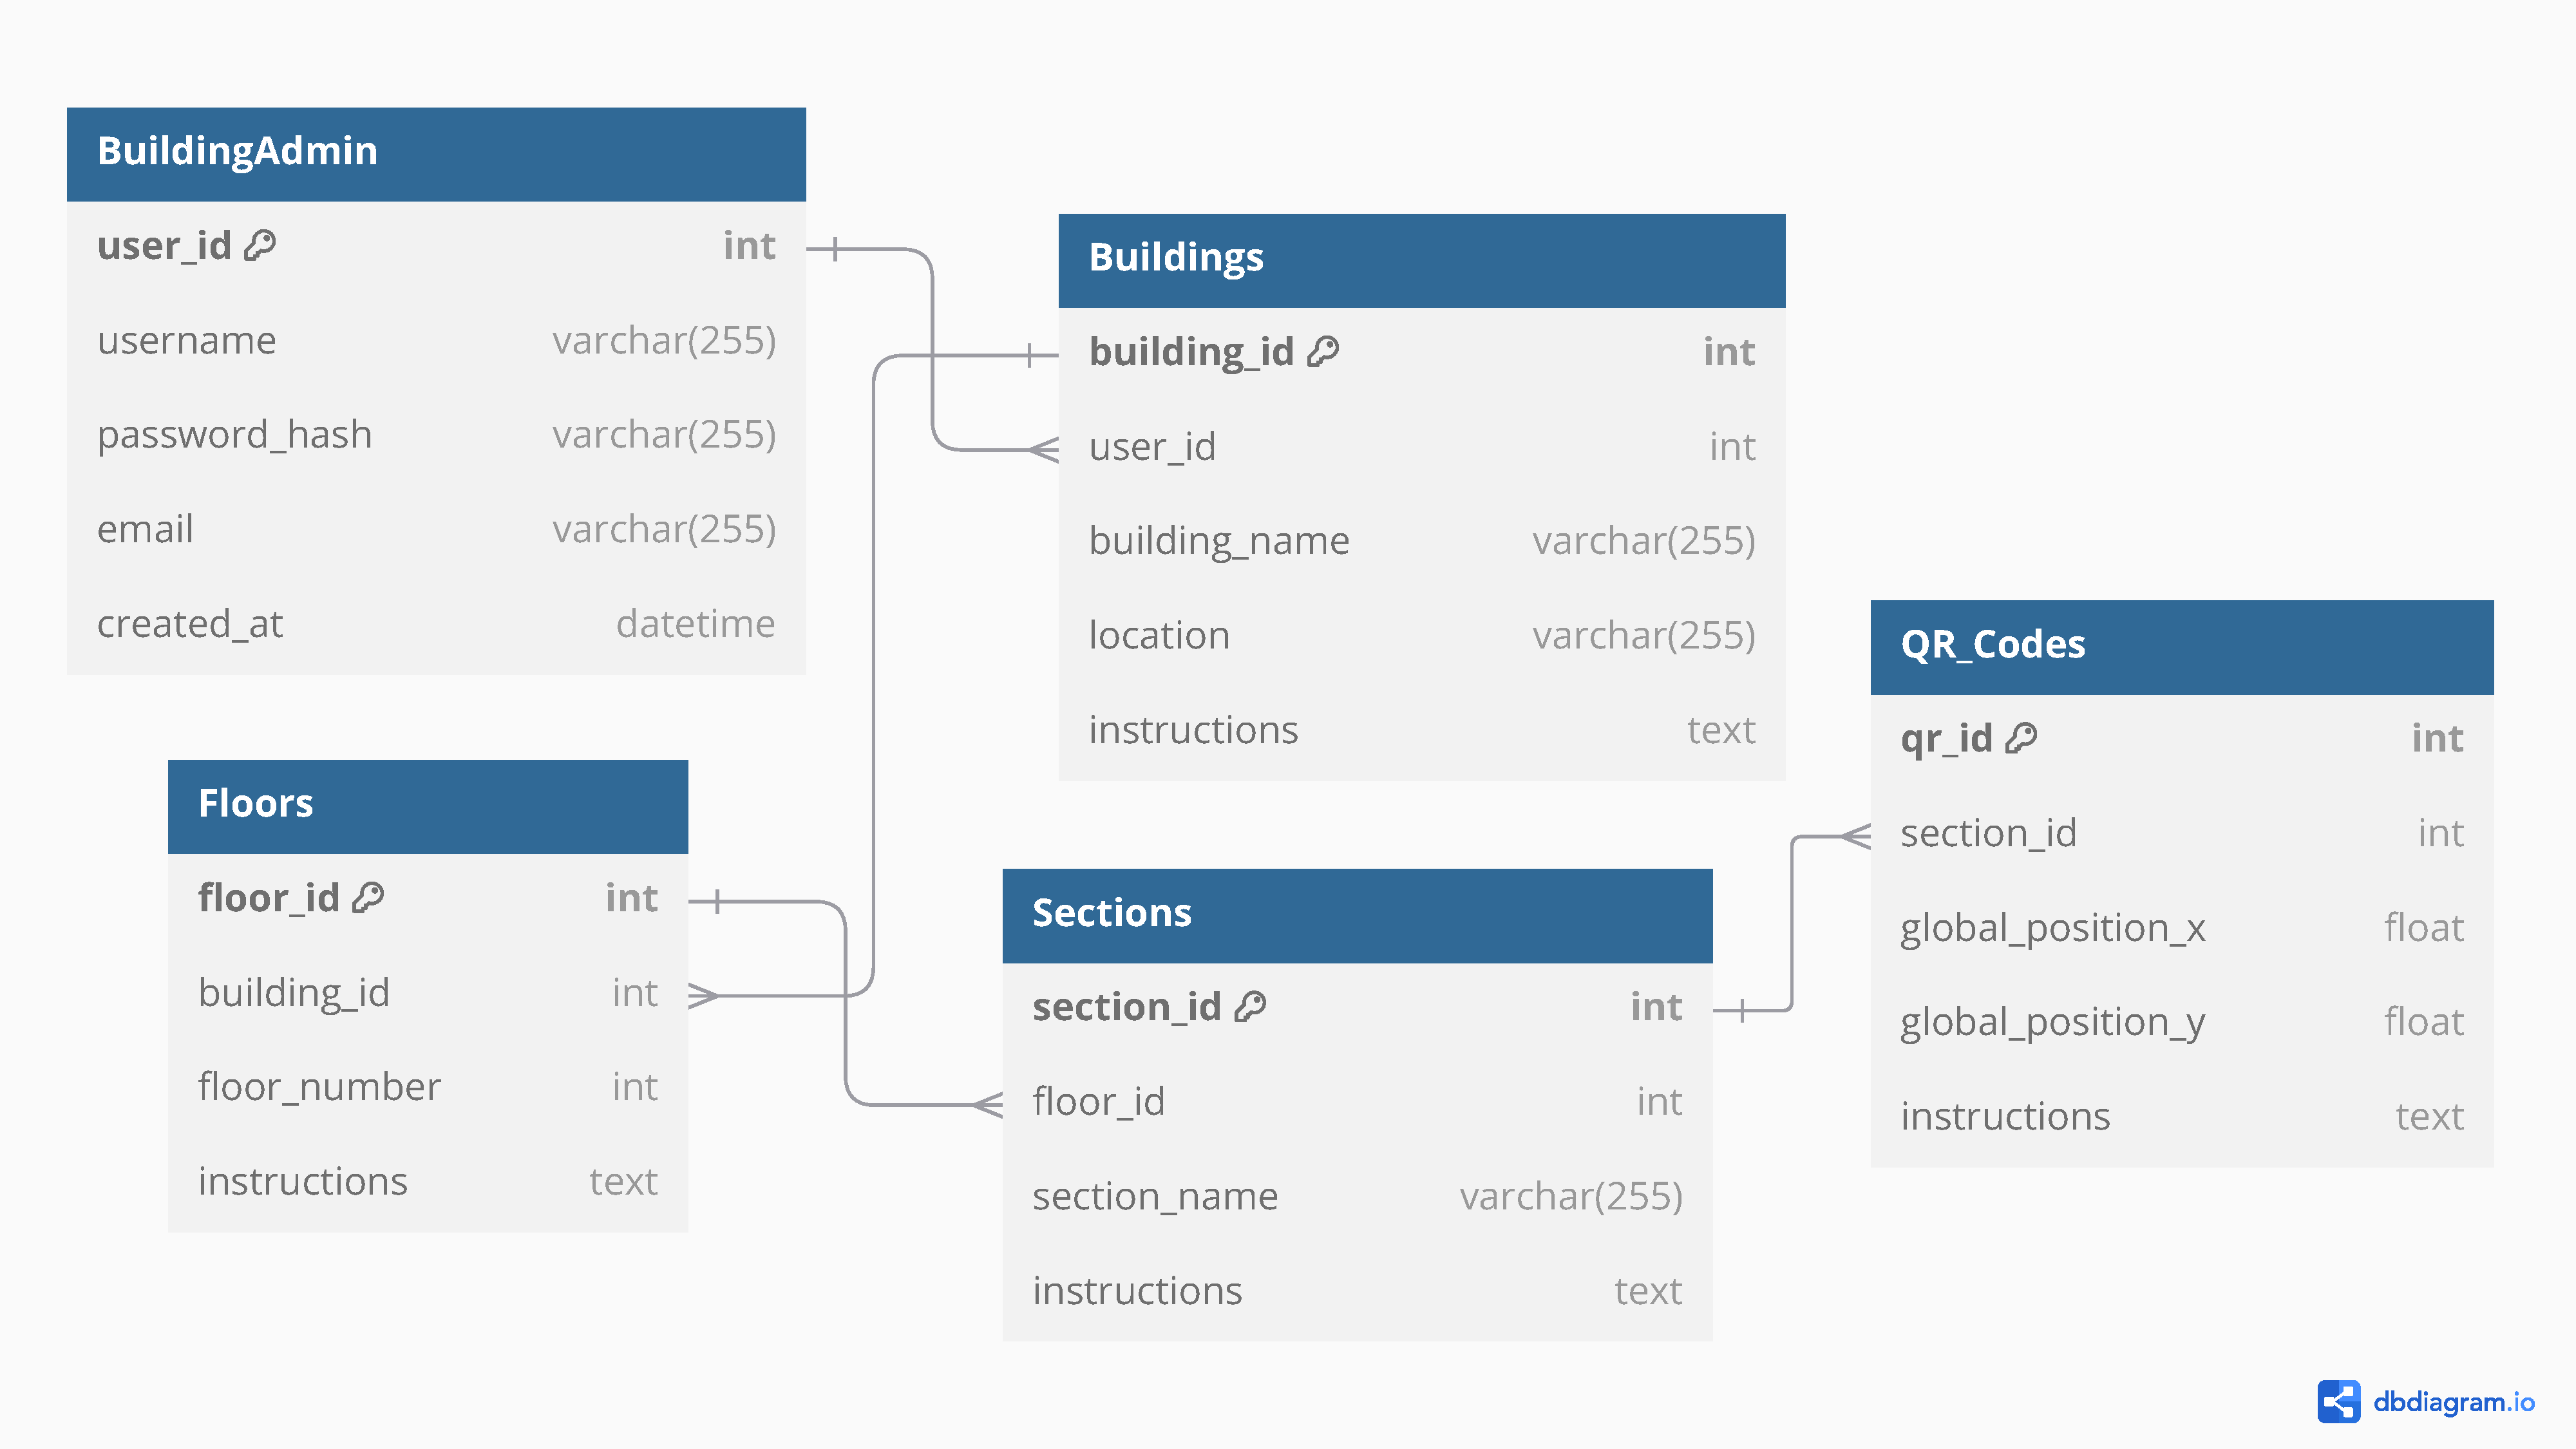
\includegraphics[width=1\linewidth]{assets/ch3/our_ERD}
	\caption{Entity-Relationship Diagram (ERD) of the Mosaned Database System}
	\label{fig:our_ERD}
\end{figure}

The database structure, shown in Figure~\ref{fig:our_ERD}, organizes data into five interconnected tables to ensure efficient management of users, buildings, floors, sections, and QR codes. By maintaining this structured hierarchy, the database supports both the localization system and the customizable guidance system, ensuring accuracy and real-time functionality.

Building managers interact with the database through a Building Management Dartboard, enabling them to configure and manage metadata such as building-specific instructions and QR code positions. The metadata and features of the database are detailed in Appendix~\ref{appendix:db_metadata}.


\section{Building Management Dashboard}

The Building Management Dashboard is a web-based tool that allows building administrators to manage the indoor navigation system effectively. This dashboard provides an interface to control and update QR code instructions and manage QR codes within the building remotely.

Key features include:
\begin{itemize}
	\item \textbf{User Authentication:} Allows administrators to securely log in and access only their managed buildings.
	\item \textbf{Building and Floor Management:} Displays a list of buildings and their respective floors, allowing administrators to organize and view all QR codes assigned to each area.
	\item \textbf{QR Code Instruction Editing:} Administrators can add, update, or delete instructions for each QR code in the building, tailoring guidance to specific areas and ensuring data accuracy.
\end{itemize}


The dashboard enables efficient oversight and maintenance of QR code-based navigation, allowing real-time updates without modifying the physical QR codes.